\documentclass[conference]{IEEEtran}
\IEEEoverridecommandlockouts
% The preceding line is only needed to identify funding in the first footnote. If that is unneeded, please comment it out.
% \usepackage{cite}
% Enables Portuguese Brasil
% \usepackage[portuguese]{babel}
%encoding
% Enables code listing
\usepackage{listings}
%--------------------------------------
\usepackage[T1]{fontenc}
\usepackage[utf8]{inputenc}
%--------------------------------------
%Enables the use of greek letter without a math context
\usepackage{textgreek}
%--------------------------------------
%Enables hiperlinks
\usepackage[hidelinks]{hyperref}
%--------------------------------------

\usepackage{amsmath,amssymb,amsfonts}
\usepackage{algorithmic}
\usepackage{graphicx}
\usepackage{textcomp}
\usepackage{xcolor}


% The code style
\usepackage{color}
\definecolor{codegreen}{rgb}{0,0.6,0}
\definecolor{codegray}{rgb}{0.5,0.5,0.5}
\definecolor{codepurple}{rgb}{0.58,0,0.82}
\definecolor{backcolour}{rgb}{0.95,0.95,0.92}

\lstdefinestyle{mystyle}{
	backgroundcolor=\color{backcolour},   
	commentstyle=\color{codegreen},
	keywordstyle=\color{magenta},
	numberstyle=\tiny\color{codegray},
	stringstyle=\color{codepurple},
	basicstyle=\footnotesize,
	breakatwhitespace=false,         
	breaklines=true,                 
	captionpos=b,                    
	keepspaces=true,                 
	numbers=left,                    
	numbersep=2pt,                  
	showspaces=false,                
	showstringspaces=false,
	showtabs=false,                  
	tabsize=2
}
\lstset{style=mystyle}
%---------------------------------------


\def\BibTeX{{\rm B\kern-.05em{\sc i\kern-.025em b}\kern-.08em
    T\kern-.1667em\lower.7ex\hbox{E}\kern-.125emX}}
\begin{document}
\title{Classification of Histopathological Images of Breast Cells between Malignant and Benign Tumors based on Handcrafted Feature Extraction}
\author{Hiago Matheus Brajato \& André Furlan - UNESP - Universidade Estadual Paulista "Júlio de Mesquita Filho"}
\date{2019-11-14}
\maketitle

\begin{abstract}
According to the recent survey published by the International Agency for Research on Cancer (IARC), the breast cancer is one of the most common kinds of cancers diagnosed in the population nowadays. The diagnosis of this type of disease is usually made through the analysis of the breast cells by a specialist after the biopsy and staining, normally made by the combination of hematoxylin and eosin (H \& E). This manual assessment is a time-consuming task and depends on the expertise and perception of the pathologists. In order to overcome this limitations, image processing can be considered as great aid alternative. In this paper is presented an application for the classification of breast cell images between malignant and benign tumors. The developed software includes the principals steps present within the image processing field, such as preprocessing, segmentation, feature extraction and classification, in order to achieve good results in the analysis of a dataset composed by 50 images of malignant and benign tumors.
\end{abstract}

\begin{IEEEkeywords}
Breast Cancer, Image Processing, Diagnosis, Malignant and Benign
\end{IEEEkeywords}

\section{Introduction}
\par Breast Cancer is a kind of malignant tumor in which cells in the breast grow out of control. In a recent survey called GLOBOCAN \cite{GLOBOCAN} published in 2018 by the IARC, can be visualized the statistics about this type of cancer around the world. The study states that the breast cancer is the second most incident type of cancer in world, with 2 088 049 cases of this disease in the last year, and the number of cases of mortality is equals to 626 679 (about 30\% of total). According to the same study, the breast cancer is the most incident type in Brazil, with 85 620 registered cases in total, and the second most reason of mortalities among the cancers, with 18 842 cases, what represents 22\% of the total cases of breast cancer in Brazil. Figures 1 and 2 in the right graph the information presented until now. In the first chart is possible to visualize the statistics about the world, and in the second one is presented the numbers of cases in Brazil.

\begin{figure}[h]
    \centering
    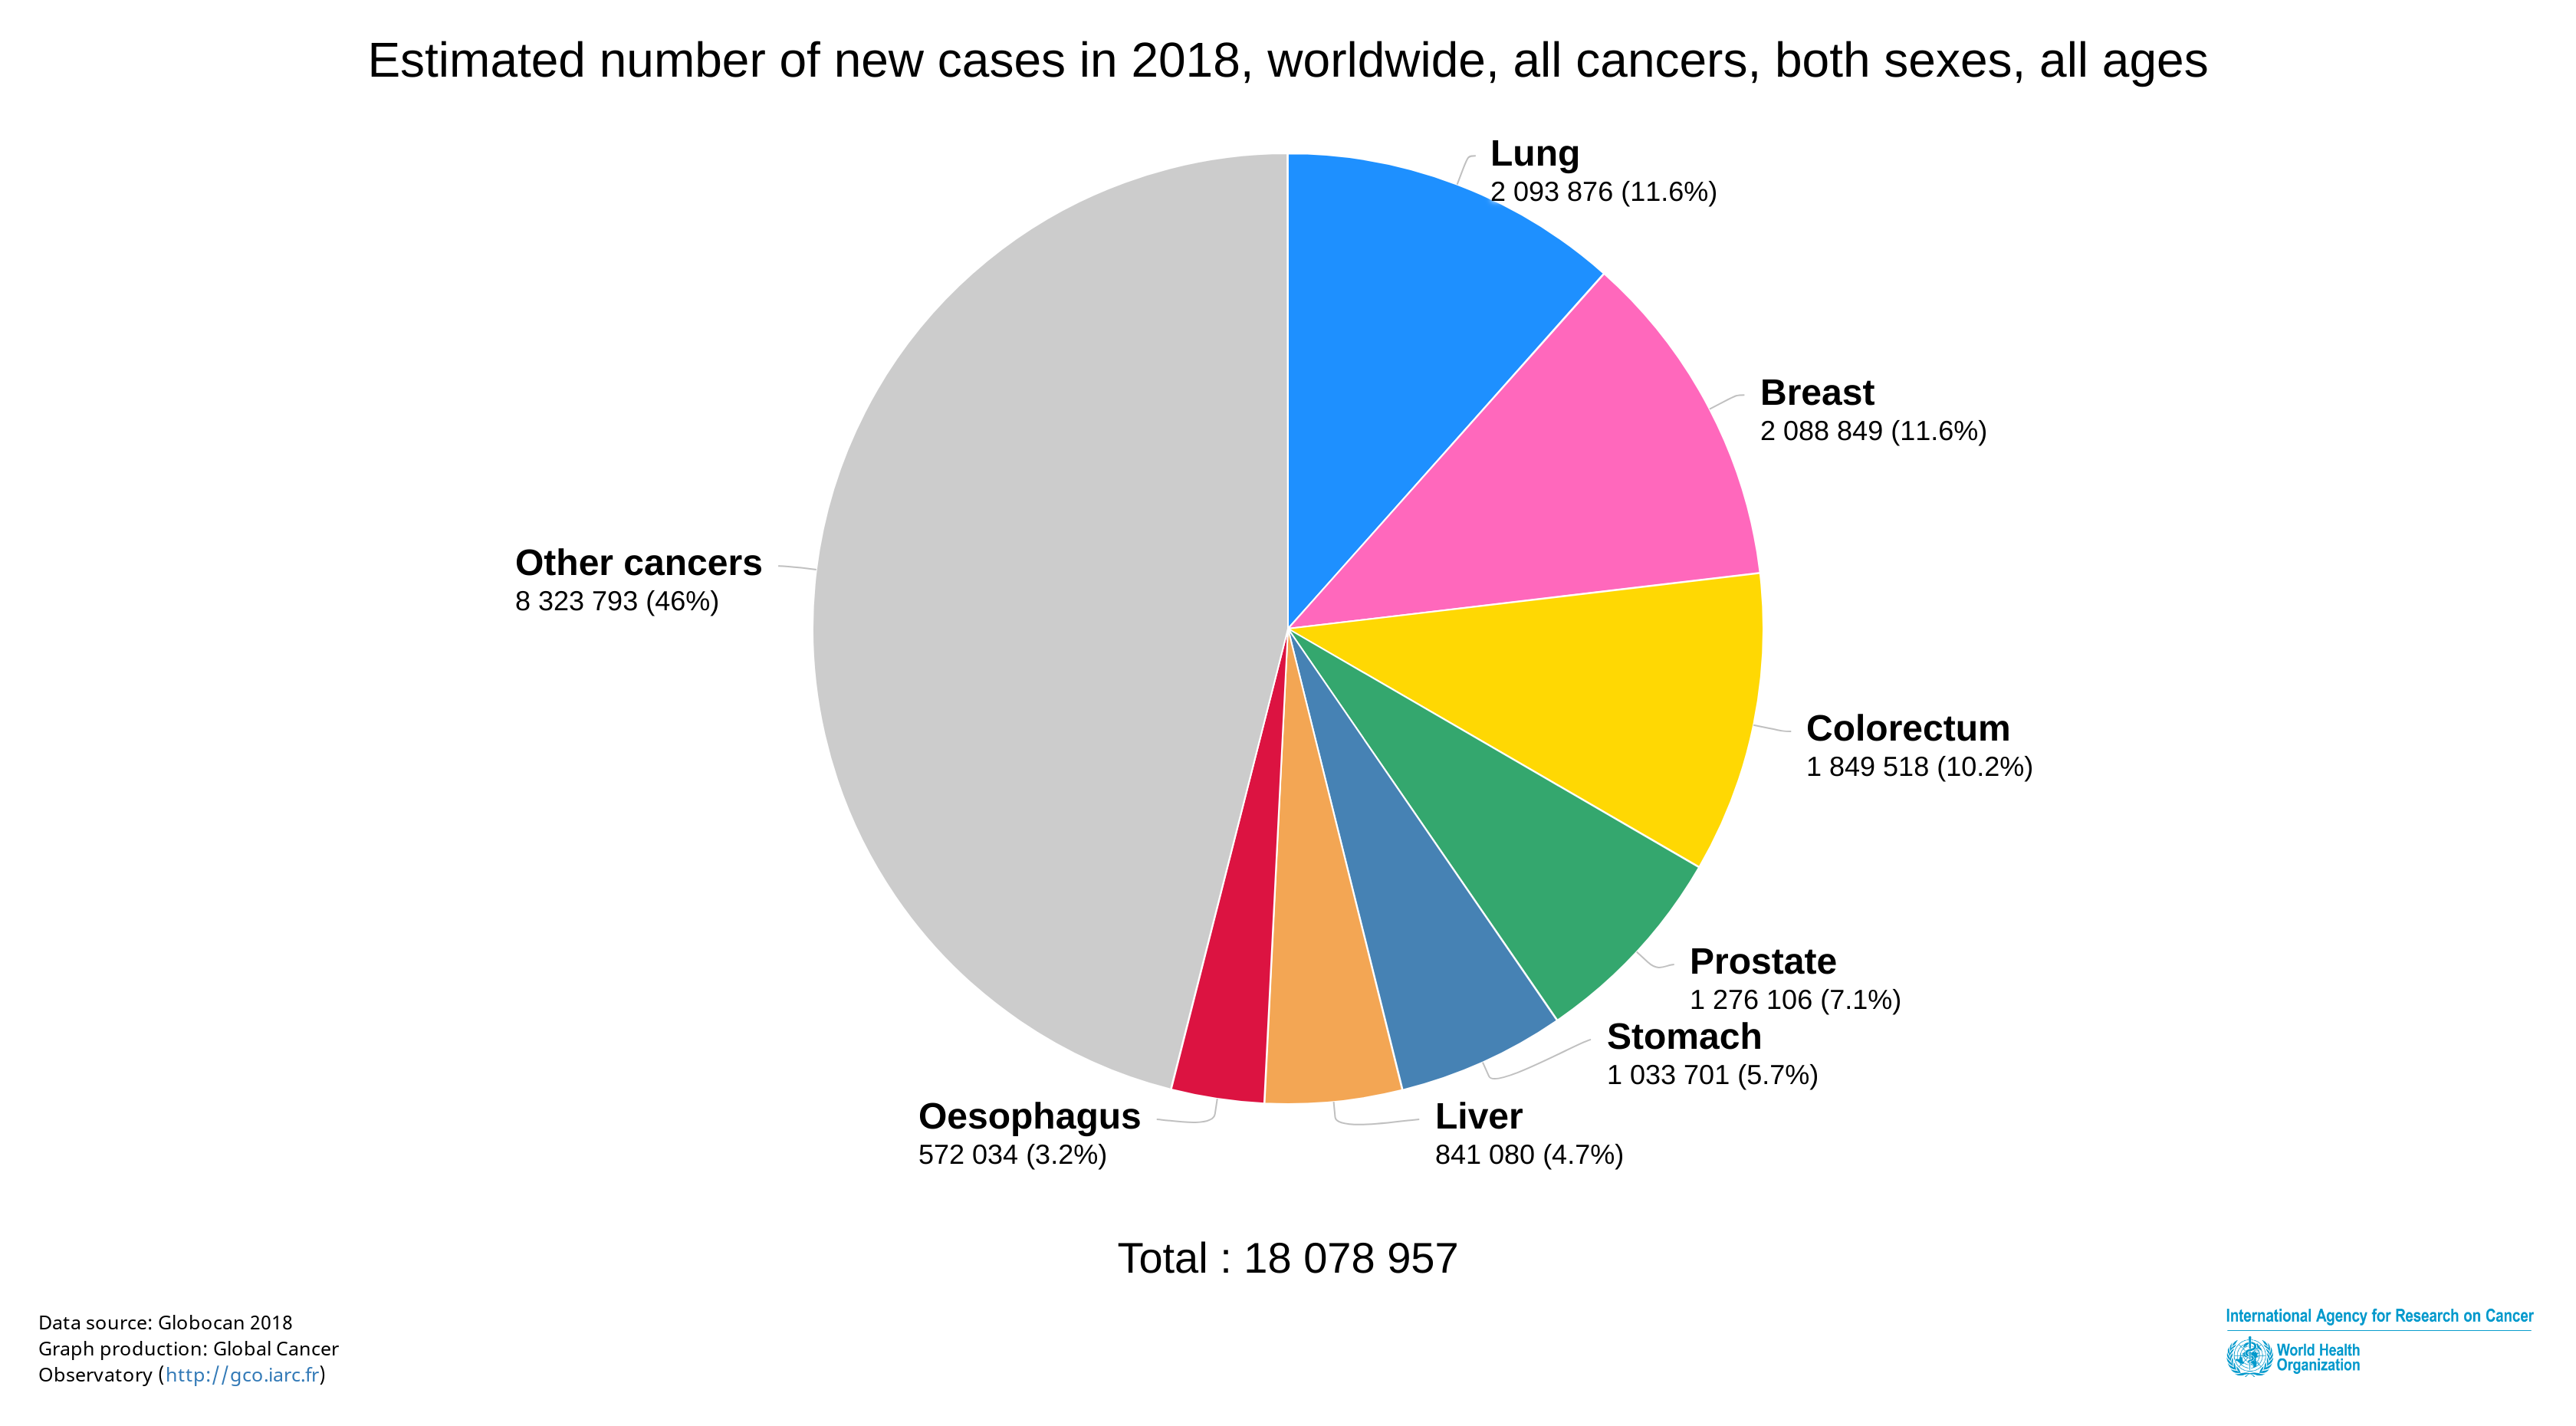
\includegraphics[width=8cm]{images/graphic1.png}
    \caption{Statistics about Incidence of types of Cancer in the World \cite{GLOBOCAN}}
    \label{fig:my_label}
\end{figure}

\begin{figure}[h]
    \centering
    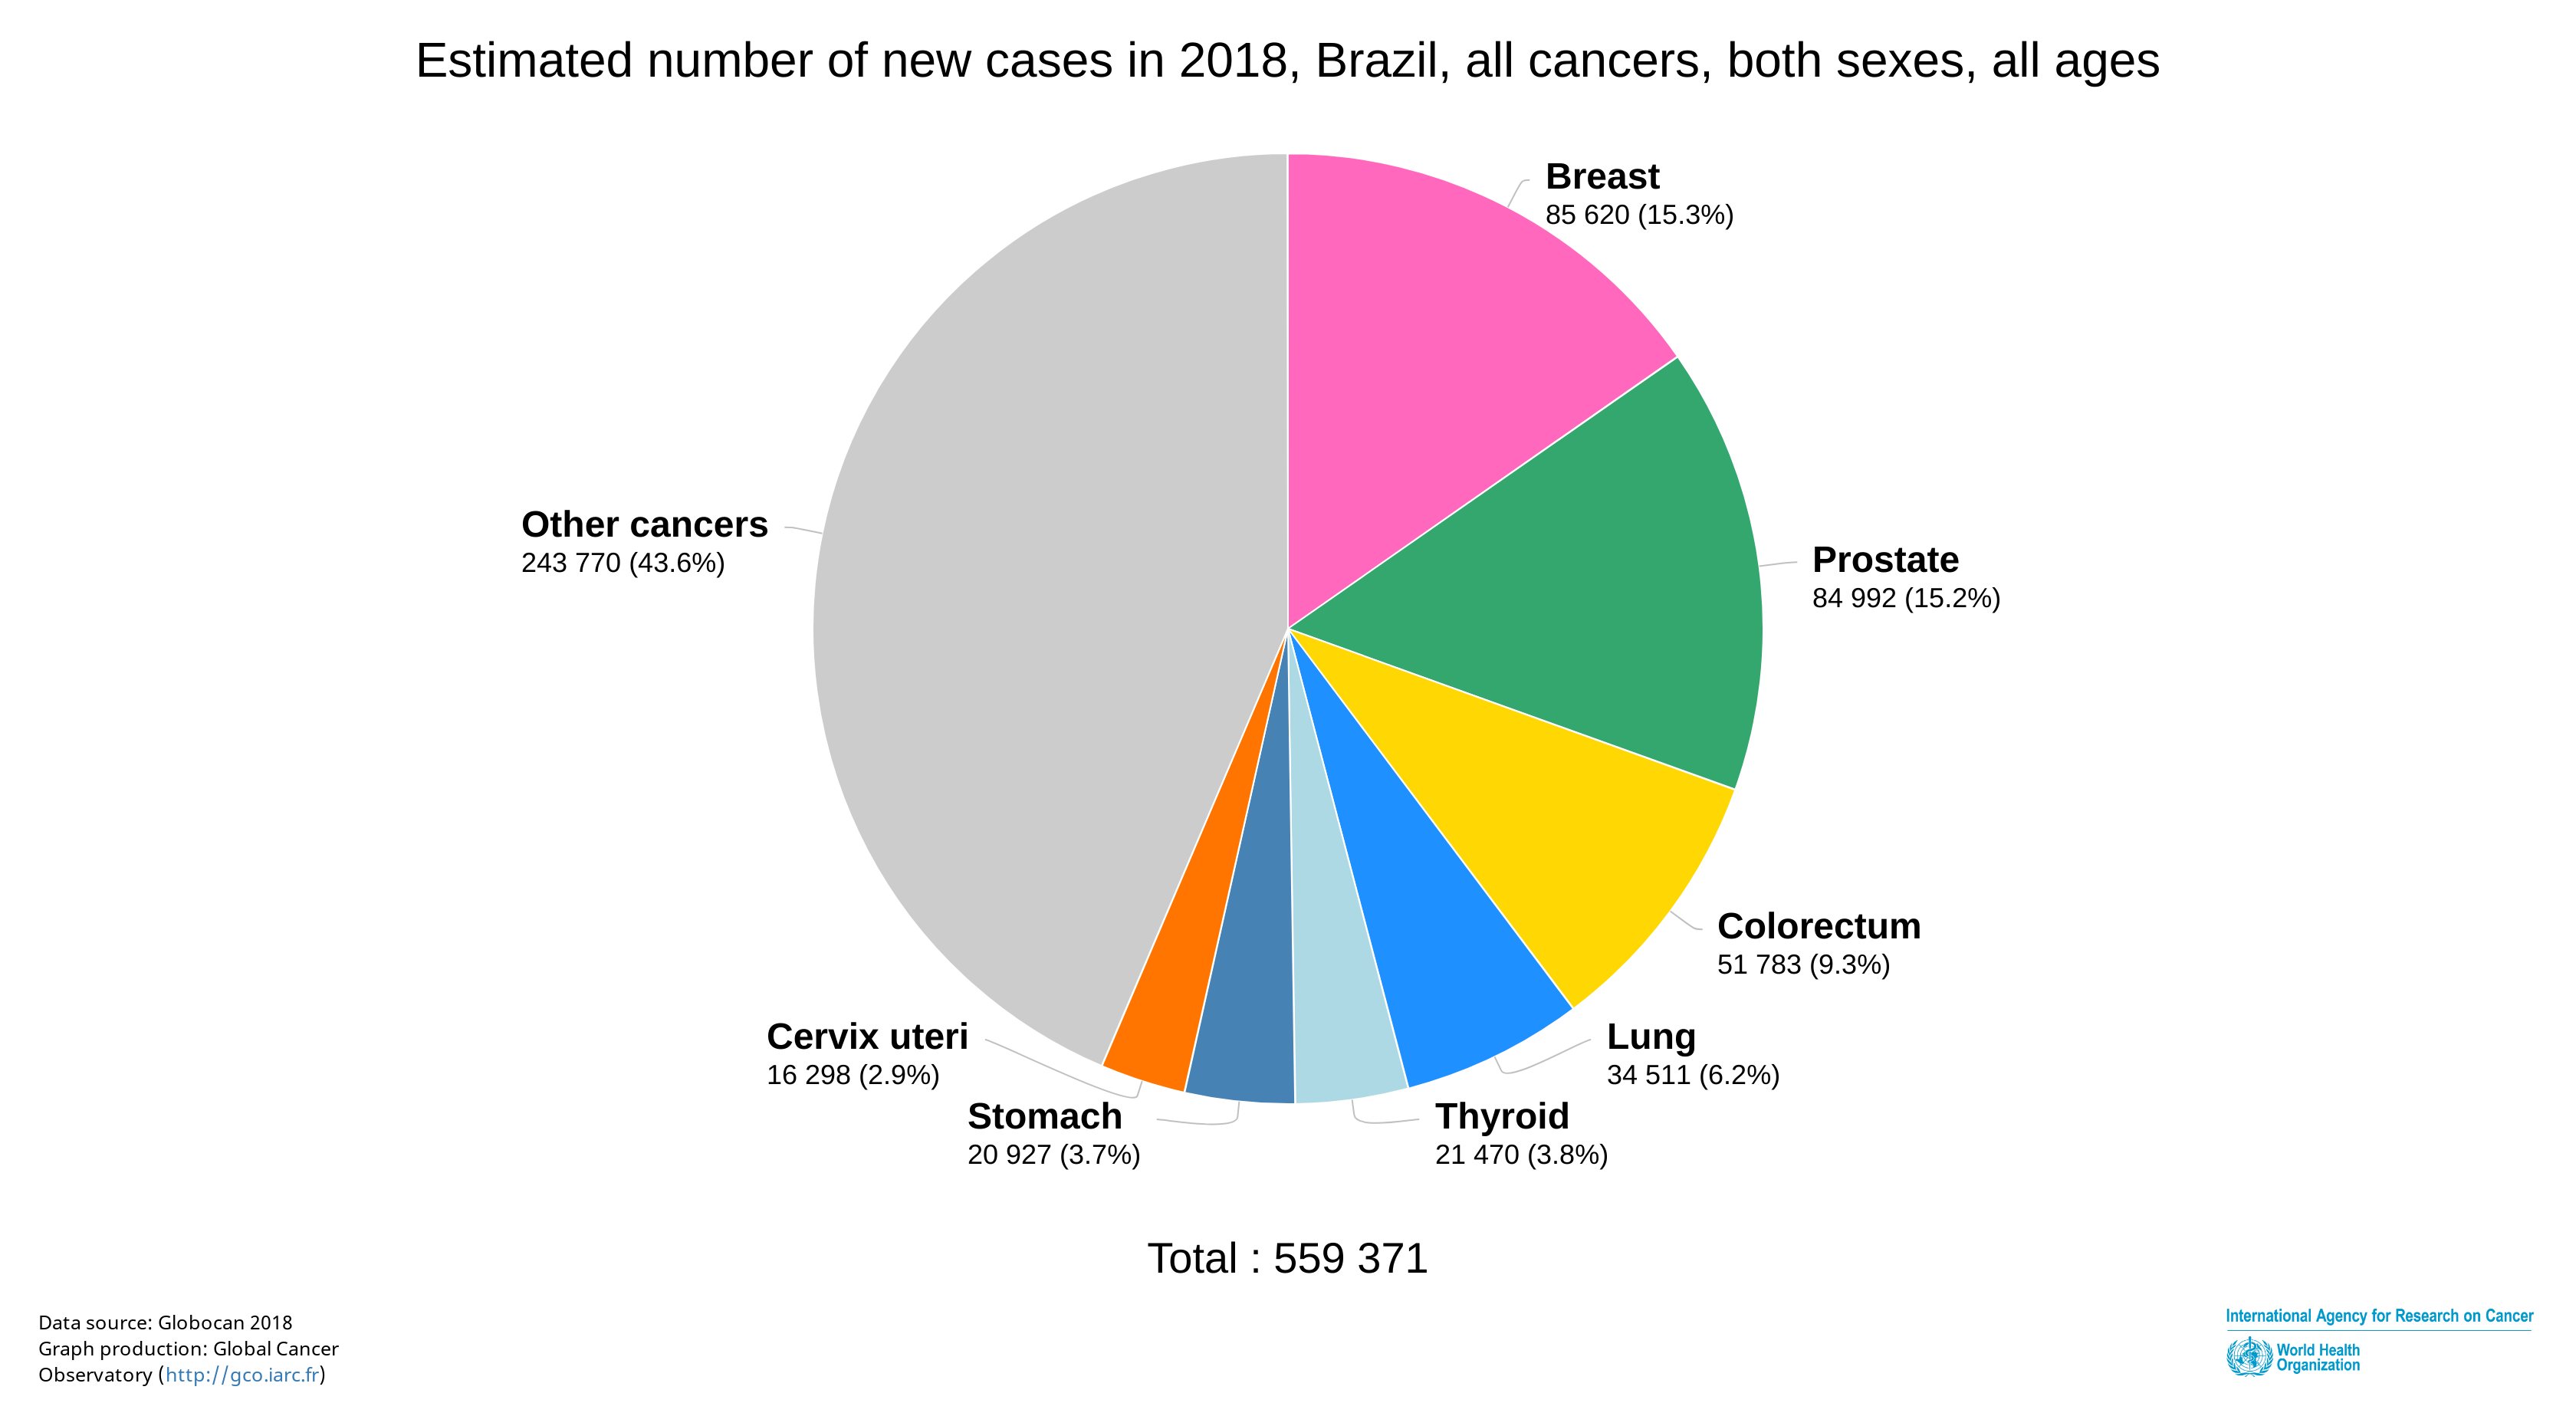
\includegraphics[width=8cm]{images/graphic2.png}
    \caption{Statistics about Incidence of types of Cancer in Brazil \cite{GLOBOCAN}}
    \label{fig:graphic2}
\end{figure}

\par The process of the diagnosis of this type of cancer is usually made by a specialist called pathologist, who is responsible for analysing breast cells acquired through two steps: biopsy and staining. The biopsy step is a test that removes tissues or fluids from the suspicious breast area, and this procedure is the only one that can definitely define if the suspected area is cancerous or not. The staining step is responsible for add color to the cells in order to become easier the visualization of the tissue by the pathologist. After this two steps, the specialized doctor analyses the tissue through a microscope in order to determine if the there are malignant tumors or benign ones. As can be seen, the diagnosis is a really time-consuming task, which depends strongly of the expertise of the specialist. Therefore, is interesting the possibility of having applications that analyse digital images of this breast cells and be able to assist the doctor in the process of diagnosis. 

\par The Digital Image Processing is the computational field responsible for dealing with this kind of task, which involves some steps for processing the image in order to achieve the better possible classification rate, in this case between malignant and benign tumors. This paper presents the steps present within of the development of an application responsible for classifying images of breast cells from features extracted, which will be described in the sequence of the paper. Some measures as accuracy, ROC Curve and AUC are compared in order to indicate the best combination of features and classifier. The rest of the paper is organized as follow:  Section II is responsible for presenting the image acquisition, while the section III demonstrates how the filtering of the images was made. Section IV presents the segmentation step, and its impact in the following phases. The step of feature extraction is presented in Section V and the feature selection in Section VI. Finishing the paper, the Section VII presents the process of classification, while Sections VIII and IX present the results and conclusion respectively.

\section{Image Acquisition}
\par The used dataset in this work is composed by 50 images of breast cells, being that 24 images are of malignant tumors and 26 of benign ones. Informations about this dataset can be found in \cite{artigo_database} and \href{https://bioimage.ucsb.edu/research/bio-segmentation}{\textbf{https://bioimage.ucsb.edu/research/bio-segmentation}}. The Figure 3 below presents a flowchart of the sequence of steps developed in the application.

\begin{figure}[h]
    \centering
    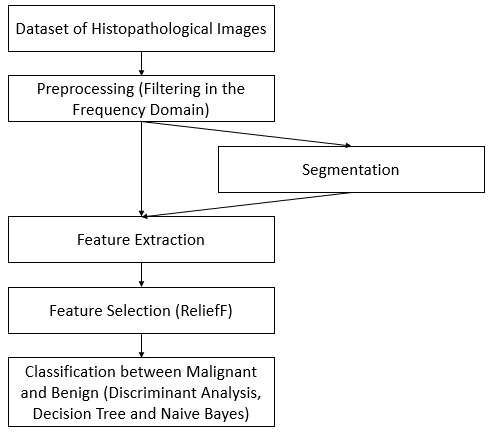
\includegraphics[width=8cm]{images/imagem3.png}
    \caption{Flowchart of the developed method}
    \label{fig:my_label}
\end{figure}

\section{Filtering: Frequency Domain}
\par The main objective of this section is separate from the noisy background the interesting areas, so the classifiers do not need to evaluate irrelevant data.
The main idea behind it is to subtract the low frequencies components from the image and, using morphological operations, remove remaining noises and close the gaps.
\subsection{Filtering and masking}
	Two kinds of filters were used:
	\par A low pass filter, witch is used to highlight the low frequencies features of the image, with radius of  empirically determined 50 pixels, and a high pass filter, to enhance the detailed information at the image, with  radius of one.
	
	\par To get the mask (figure \ref{fig:mask}) a simple subtraction operation of grayscaled lowpass filtered image from highpass filtered image is made and ,on the resulted image, Otsu thresholding operation is applied followed by three morphological operations: An erosion using a circle mask of three pixels, a dilation using a circle mask of five pixels and a hole filling; these values were empirically chosen to get rid of noisy information in the image and avoid to hide important features of the image.
	
	\begin{figure}[h]
		\centering
		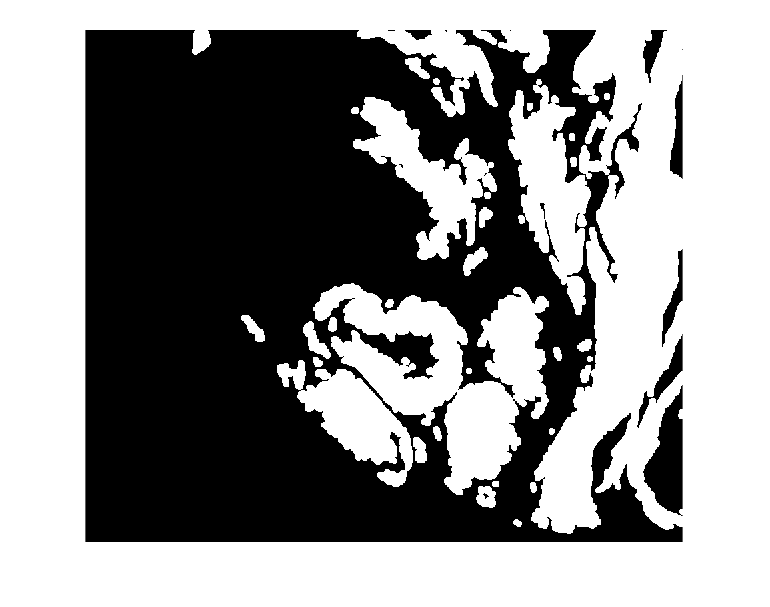
\includegraphics[width=0.7\linewidth]{images/fourrierFiltering/mask}
		\caption{Image mask generated}
		\label{fig:mask}
	\end{figure}

	\par Now that mask is ready, this one is applied to the original image (figure \ref{fig:original}), the result of that operation is that the area with white pixels are shown and the area with black pixels are hidden (figure \ref{fig:maskedimage}).

	\begin{figure}[h]
		\centering
		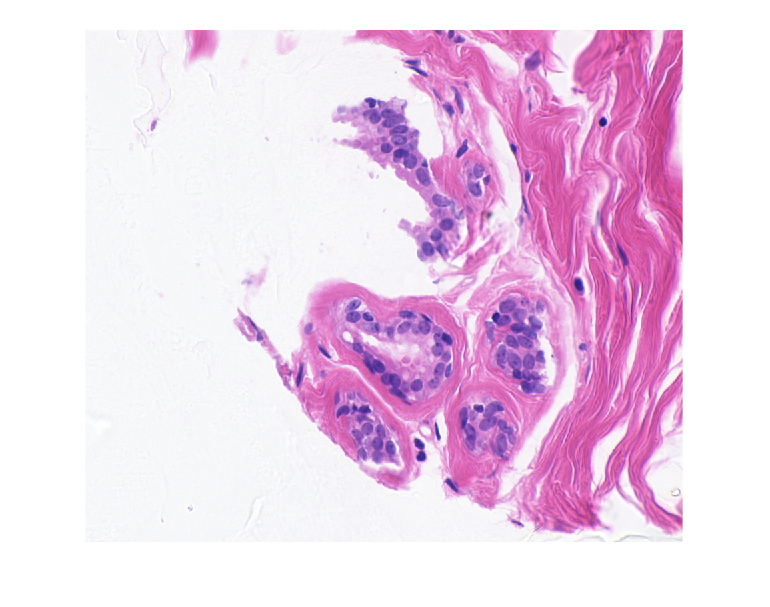
\includegraphics[width=0.7\linewidth]{images/fourrierFiltering/original}
		\caption{Original image}
		\label{fig:original}
	\end{figure}

	\begin{figure}[h]
		\centering
		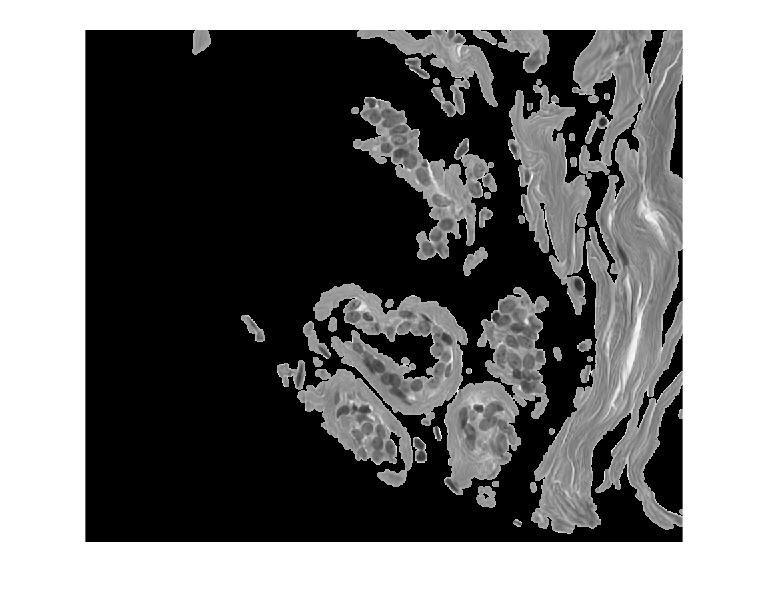
\includegraphics[width=0.7\linewidth]{images/fourrierFiltering/maskedImage}
		\caption{Image with mask}
		\label{fig:maskedimage}
	\end{figure}
\section{Segmentation}
\par The segmentation is an important step within the image processing, which is responsible for subdividing  an image in regions or objects that compose the signal \cite{Gonzalez:2006:DIP:1076432}, usually, this process is made through the separation of the image between background and object. Several techniques can be used in this process, such as based on thresholding, edge detection, region approaches. In this work, the optimal thresholding technique called Otsu was chosen due to its simplicity and good results. The segmentation was made after the filtering step, and the approach taken in the present work is to subtract the background of the segmented image from the original gray levels image. The code responsible for doing this task and the result produced in the image are shown in the Figure 4.

\begin{figure}[h]
    \centering
    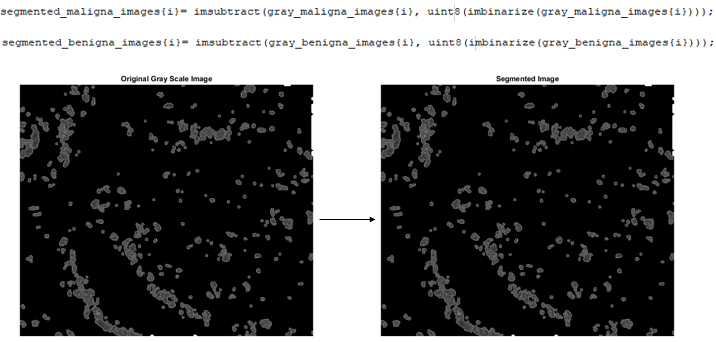
\includegraphics[width=8cm]{images/imagem_segmentacao.png}
    \caption{Segmentation of an Image of Malignant Tumor}
    \label{fig:imagem_segmentacao}
\end{figure}

\par Although visually is difficult to realize differences between the original image and the segmented one, was checked during the tests that for this image 223 682 pixels were modified in the resulted image in comparison with the original one. Since the dataset is composed for images of resolution 896x768, this quantity of modified pixels achieve around 32\% of the total.

\par Before proceeding for a description of the next steps, it is important to say that the segmentation step is not always necessary in image processing; usually, this step is applied when the following steps as feature extraction and classification are not presenting good results and it is needed to improve the process.\par
Taking this in consideration, in the next sections is presented some measures of classification for segmented and non segmented images, in order to determine the importance and necessity of this step in the whole process.

\section{Feature Extraction}
The Feature Extraction can be considered as one of the most important steps in Image Processing: this is the last phase before the classification of the samples. So, the main objective here is to compose feature vectors capable to describe the samples, in order to classify correctly each example in its real class.\par
Commonly, two approaches can be chosen in order to extract descriptors from an image: Handcrafted Features and Non-Handcrafted ones. The Handcrafted Features, as the name claims, are the descriptors extracted manually, according to choice of the developer, while the Non-Handcrafted Features are extracted in an automatic way, in order to do the best possible classification (one example of this approach are the Convolutional Neural Networks - CNN). \par
As mentioned in the title of this paper, the used approach for extracting the descriptors from the histopathological images was the handcrafted one, where 11 descriptors were extracted and used as the input of the classifiers. It is important to remember that the extraction was accomplished from segmented images and non-segmented ones, so, it is possible to compare the impact of the segmentation step during the classification. Below is presented the extracted features used in the process.\par
The descriptors used in the present process can be divided into 3 categories: First Order Measures, Second Order Measures and Others. The First Order Measures are the descriptors that consider just the gray level information about the pixels, not considering the spatial relation among them. The Second Order Measures, instead of the first ones, consider the spatial relation among the pixels, beyond the gray level property. These descriptors are extracted from the called Gray Level Co-occurrence Matrix (GLCM), that is responsible to store the frequency that a pixel with gray level \textbf{i} and other with gray level \textbf{j} occur in the image, separated for a distance \textbf{d}, in the direction\textbf{ $\theta$} \cite{conci2008computacao}. This method was proposed in 1973 by \cite{haralick:smc1973}, and the descriptors extracted from the GLCM are called Haralick descriptors (in the present work 6 of the 14 descriptors proposed by Haralick were used).\par
The ther group mentioned in the paragraph above includes the descriptors that do not fit the First and Second Measures, so, becomes important to explain how these descriptors were extracted in the proposed method. Three descriptors can be found in this last group: Fourier Descriptors, Local Binary Pattern Features and Fractal Dimension Descriptors. \par
The Fourier Descriptors (FD), as the name say, are the features extracted from the Fourier Transform, that is responsible to transform the visualization of the signal from the spatial domain to the frequency domain, in order to become possible to see the frequencies that compose the image. Different approaches can be chosen to extract the FD`s, in the present work the proposed process was as follows:
\begin{itemize}
    \item The image was transformed to the frequency domain with the Fast Fourier Transform (FFT).
    \item Without doing the shift of the transformed, a number of N coefficients in the middle of the spectrum were taken, so just the high frequencies was caught from the FFT. Doing this process, it is possible to reconstruct the image just with these high frequencies coefficients, that represent the edges inside the signal. In the Figure 8 it is possible to see the original image and the reconstructed one made from the descriptors.
    \item Lastly, the complex magnitude was computed for the coefficients.
\end{itemize}{}

\begin{figure}[h]
    \centering
    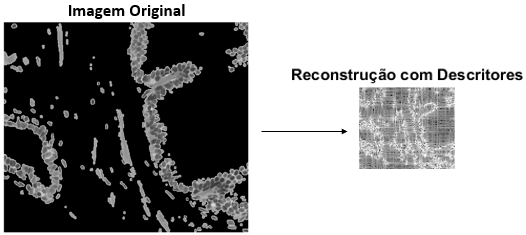
\includegraphics[width=8cm]{images/imagem_reconstrucao.png}
    \caption{Original Image and its reconstruction using the Fourier Descriptors}
    \label{fig:my_label}
\end{figure}{}
The Local Binary Pattern Features (LBP) was described in \cite{lbp-OjalaPH96}, being a two-level version of the Texture Unit model proposed by \cite{Wang:1990:TCU:83597.83606}. The main idea is describe the image considering a neighborhood of 3x3 pixels and comparing the gray levels.\par
The Fractal Dimension Descriptors extracted in the present work were obtained using the Box Counting Theorem, a method where the image is divided into N windows according to a certain scale and the number of boxes that contains the objects that must be counted. Doing this, it is possible to obtain the Fractal Dimension from each scale, as well as a General one calculated through the angular coefficient.\par
The Figure 9 summarizes the descriptors obtained in the present work. 
\begin{figure}[h]
    \centering
    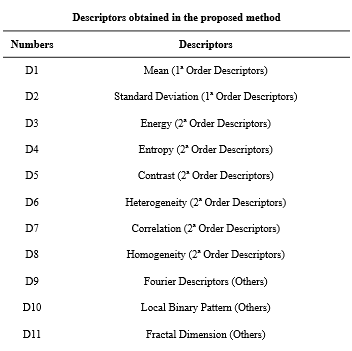
\includegraphics[width=8.5cm]{images/table_descriptors.png}
    \caption{Descriptors}
    \label{fig:my_label}
\end{figure}{}

\section{Feature Selection}
The feature vector composed in the last step is formed by all descriptors presented in Figure 9, but it is not a good idea providing the feature vectors with all attributes as input to the classifiers, because the probability of the classification does not achieve good results is large doing the process in this way. This can be explained from the problem so-called "Curse of Dimensionality": after a certain number of descriptors, increasing the length of the feature vector with more attributes can degrade the performance of the classifiers.\par
In order to obtain the more relevant descriptors and the best number of attributes, the feature vector with 7175 descriptors was examined by the ReliefF method, which is responsible for ranking the importance of the predictors based on its capability of distinguishing samples of different classes. The next section presents the analysis made by the ReliefF, taking into consideration the performance of the classifiers.


\section{Classification}
The relevance of the descriptors, as well the performance of the classifiers were measured by the analysis of ROC Curve and area under curve ROC (AUC). This measures were used in the proposed method because the malignant an benign classes are unbalanced in dataset, considering that there are 24 malignant samples and 26 benign ones. Taking this is consideration, it is not a good idea analysing the obtained results through measures as accuracy, because the calculation of this last measure does not take the class balancing into consideration.\par
The ROC Curve and AUC allow to analyse the performance of the classifiers through the confusion matrix obtained varying the threshold, so the plotted graph is formed by the X axis (1 - Specificity) and Y (Sensitivity), therefore, the AUC with value equals to 1 represents a perfect classification, while an AUC equals to 0.5 or less represents a random classification.\par
The performance of the proposed method was evaluated through the classifiers \textbf{Discriminant Analysis}, \textbf{Decision Tree} and \textbf{Naive Bayes}, taking into consideration that all of these classifiers were submitted to the K-Folds validation method, with K equals to 5.\par
The best number of descriptors found by testing the classifiers used in the present method can be seen in the Figure 10, which shows the number of descriptors used for the classification in X axis, and the average rates for AUC in the Y axis.\par
It is important to remember that the graph contained in the Figure 10 was obtained using the segmented images in the process; the best number of descriptors obtained (35) was also tested in the same process without the segmentation step, in order to determine the importance of this phase in the whole process. The AUC rates obtained for the Discriminant Analysis, Decision Tree and Naive Bayes were 0.83, 0.66 and 0.75 respectively, resulting in an average of 0.746, well below the value showed in the graph (0.823). This information show us that the segmentation step produces a significant improvement in the performance of the classifiers, being necessary use its during the proposed method.

\begin{figure*}[h]
    \centering
    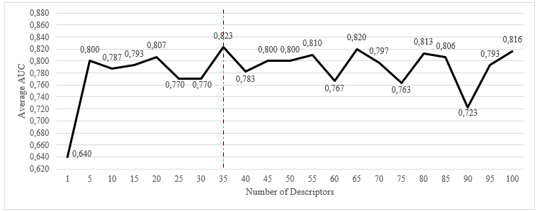
\includegraphics[width=18.3cm]{images/chart.png}
    \caption{Average rates for AUC varying the number of descriptors taking into consideration the classifiers: Decision Tree, Discriminant Analysis and Naive Bayes}
    \label{fig:my_label}
\end{figure*}{}

\section{Results}
	\par The classifiers used 
discrim analysis
decision tree
naive bayes

Acurácia média de classificação: 0.763232
Acurácia média de classificação: 0.720606
Acurácia média de classificação: 0.676566
lorem ipsum, lorem ipsum, lorem ipsum, lorem ipsum, lorem ipsum, lorem ipsum, lorem ipsum, lorem ipsum, lorem ipsum, lorem ipsum, lorem ipsum, 

\section{Conclusion}
lorem ipsum, lorem ipsum, lorem ipsum, lorem ipsum, lorem ipsum, lorem ipsum, lorem ipsum, lorem ipsum, lorem ipsum, lorem ipsum, lorem ipsum, 

\bibliographystyle{plain}
\bibliography{references.bib}
\end{document}